\documentclass[a4paper,10pt]{article}
\usepackage{tikz}
\usepackage{fullpage}
\usepackage{amsmath,amsthm,amsfonts,amssymb,amscd}
\usepackage{mathtools}
\usepackage{colortbl}
\usepackage{xcolor}
\usepackage{graphicx}
\usepackage{titlesec}
\usepackage{xepersian}
\usepackage{multirow}
\usepackage{caption}
\usepackage{fancyhdr}
\usepackage{mdframed}



% ---------------------------
%      Color Palette
% ---------------------------
\definecolor{BgDark}{HTML}{141420}
\definecolor{BgCard}{HTML}{1E1E2E}
\definecolor{AccentBlue}{HTML}{7AA2F7}
\definecolor{AccentPurple}{HTML}{BB9AF7}
\definecolor{AccentCyan}{HTML}{7DCFFF}
\definecolor{AccentGold}{HTML}{E0AF68}
\definecolor{TextPrimary}{HTML}{CDD6F4}
\definecolor{TextMuted}{HTML}{6C7086}
\definecolor{RuleLine}{HTML}{313244}

\definecolor{NodeLight}{HTML}{5B9BD5} % Standard light blue nodes
\definecolor{NodeDark}{HTML}{26527C}  % Darker blue nodes (A, E)
\definecolor{NodeGreen}{HTML}{00B050} % Green goal node (M)
\definecolor{EdgeLine}{HTML}{F4B183}  % Orange/Peach colored edges

\pagecolor{BgDark}
\color{TextPrimary}


% ---------------------------
%  RTL-safe Info Box
% ---------------------------
\newmdenv[
backgroundcolor=BgCard,
fontcolor=TextPrimary,
linecolor=AccentBlue,
linewidth=1.2pt,
rightline=true,   % RTL: accent border on the RIGHT
leftline=false,
topline=false,
bottomline=false,
innerrightmargin=12pt,
innerleftmargin=12pt,
innertopmargin=10pt,
innerbottommargin=10pt,
skipabove=10pt,
skipbelow=10pt,
]{infobox}
% ---------------------------
%        Font Setup
% ---------------------------
\settextfont{Vazir.ttf}[
    BoldFont = Vazir-Bold.ttf,
    Path = fonts/
]
\setlatintextfont{Vazir.ttf}[
    BoldFont = Vazir-Bold.ttf,
    Path = fonts/
]

% ---------------------------
%     Custom Adjustments
% ---------------------------
\renewcommand{\baselinestretch}{1.2}
\renewcommand{\thesection}{\arabic{section}}

% User-defined commands for homework info (adjust as needed)
\newcommand{\HomeworkNumber}{3}
\newcommand{\HomeworkDeadline}{1405/1/28}
\newcommand{\id}{\texttt{\detokenize{@@MhsaArl}}}



\begin{document}

% ---------------------------------
%           Title Page
% ---------------------------------
\begin{titlepage}
	
	% Background decorations — right-side rectangle + gold horizontal line
	\begin{tikzpicture}[remember picture, overlay]
		% Right-side vertical rectangle (accent block)
		\fill[BgCard]
		([xshift=-2.2cm]current page.north east) rectangle
		(current page.south east);
		\draw[AccentGold!60, line width=0.8pt]
		([xshift=-2.2cm]current page.north east) --
		([xshift=-2.2cm]current page.south east);
	\end{tikzpicture}
	
	\vspace*{2.2cm}
	
	\begin{center}
		% Logo
		
\includegraphics[scale=1.05]{assets/fum-logo.png}\\[1.0cm]
		
		\textcolor{RuleLine}{\rule{8cm}{0.6pt}}\\[0.6cm]
		
		{\Huge \bfseries \textcolor{TextPrimary}{مبانی و کاربردهای هوش مصنوعی}}\\[0.4cm]
		
		\textcolor{RuleLine}{\rule{8cm}{0.6pt}}\\[0.4cm]
		
		{\large \textcolor{AccentCyan}{دانشگاه فردوسی مشهد}}\\[0.1cm]
		{\normalsize \textcolor{TextMuted}{گروه مهندسی کامپیوتر}}\\[0.2cm]
		{\normalsize \textcolor{AccentGold}{دکتر زارعی}}\\[1.6cm]
		{\normalsize \textcolor{TextMuted}{بهار 1405}}\\[0.2cm]
		
		% Homework number — simple, normal size
		{\normalsize \textcolor{TextMuted}{تمرین شماره}}
		{\large \bfseries \textcolor{AccentBlue}{\HomeworkNumber}}\\[1.4cm]
		
		% Deadline badge — gold border
		\setlength{\fboxrule}{0.8pt}%
		\fcolorbox{AccentGold!60}{BgCard}{%
			\begin{minipage}{7cm}
				\centering\vspace{5pt}
				\textcolor{AccentGold}{\bfseries مهلت تحویل: \HomeworkDeadline}
				\vspace{5pt}
			\end{minipage}
		}\\[0.8cm]
		
		% TA box — gold border
		\fcolorbox{AccentGold!60}{BgCard}{%
			\begin{minipage}{8cm}
				\centering\vspace{5pt}
				\textcolor{TextMuted}{مسئول تمرین:} \quad \textcolor{AccentCyan}{\id}
				\vspace{5pt}
			\end{minipage}
		}
	\end{center}
	
\end{titlepage}
% ---------------------------------
%          Instructions Page
% ---------------------------------
\clearpage

\vspace*{4pt}
\begin{center}
	\colorbox{BgCard}{%
		\begin{minipage}{\dimexpr\linewidth-2\fboxsep\relax}
			\centering
			\vspace{6pt}
			{\bfseries\large \textcolor{AccentGold}{دستورالعمل‌ها}}
			\vspace{6pt}
		\end{minipage}%
	}
\end{center}
\vspace{6pt}

\begin{infobox}
	دانشجویان محترم لطفا به موارد زیر توجه فرمایید:
	\begin{itemize}
		\itemsep0.4em
		\item
		تحویل تمرین‌ها فقط از طریق سامانه آموزش مجازی دانشگاه امکان‌پذیر است.
		\item
		تمرین‌ها باید دست‌نویس، خوانا و با استفاده از خودکار آبی یا مشکی و یا به صورت دیجیتالی با استفاده از قلم نوری نوشته شوند.
		\item
		از تمرین‌های حل‌شده دیگران استفاده نکنید. پیامدهای این کار با دانشجو می‌باشد.
		\item
		نوشتن جواب آخر به تنهایی نمره‌ای نداشته و تمام مراحل حل، مشمول نمره می‌باشد.
		\item
		به دلیل موعد از پیش تعیین‌شده تمرین‌ها و برنامه درسی، امکان تمدید تمرین وجود ندارد. همچنین ارسال تمرین پس از موعد تعیین‌شده نمره‌ای نخواهد داشت.
		\item
		نحوه نام‌گذاری فایل پاسخ باید مطابق جدول~\ref{tab:file_format} و به شکل \lr{\texttt{pdf}} باشد.
	\end{itemize}
	
	\vspace{10pt}
	
	% RTL-safe table: use center environment, manual column colors
	\begin{center}
		\arrayrulecolor{RuleLine}
		\begin{tabular}{|>{\columncolor{BgCard}\centering\arraybackslash}p{3cm}|>{\columncolor{BgDark}\centering\arraybackslash}p{7cm}|}
			\hline
			\textcolor{AccentCyan}{\bfseries\lr{Format}} &
			\texttt{\lr{StudentID-Full\_Name-\#HwNo.pdf}} \\
			\hline
			\textcolor{AccentGold}{\bfseries\lr{Example}} &
			\textcolor{TextMuted}{\texttt{\lr{9876543210-Alan\_Turing-\#01.pdf}}} \\
			\hline
		\end{tabular}
		\captionof{table}{\textcolor{TextMuted}{شیوه نام‌گذاری فایل‌ها}}
		\label{tab:file_format}
	\end{center}
	
\end{infobox}


\vspace{8pt}
\textcolor{AccentCyan}{\rule{\linewidth}{0.8pt}}
% ---------------------------------
%          questions
% ---------------------------------
%%%%%%%%%%%%%%%%%%%%%%%%%%%%%%%%%%%%%%%%%%%%%%%%%%%%%%%%%%%%%%%%%%%%%%%%%%%%%%%%%%%%%%%%%%%%%%
\section{\textcolor{AccentGold}{سوال اول}}
با توجه به الگوریتم شبیه‌سازی ذوب فلزات به سوالات زیر پاسخ دهید.

\begin{enumerate}
	\item[(الف)] هرگاه در میانه الگوریتم بخواهیم هر چه سریع‌تر به همگرایی برسیم، چه تغییری در شیوه تغییر دما را پیشنهاد می‌کنید؟ چرا؟
	
	\item[(ب)] در صورتی که بدانیم در دورنمای فضای حالت اکسترمم محلی نداریم، کدام یک از الگوریتم‌های شبیه‌سازی ذوب فلزات یا تپه‌نوردی را پیشنهاد می‌کنید؟ چرا؟
	
	\item[(ج)] در صورتی که الگوریتم شبیه‌سازی ذوب فلزات مدام در اکسترمم‌های محلی گیر کند، برای بهبود عملکرد الگوریتم چه راه حلی پیشنهاد می‌دهید؟ چرا؟
\end{enumerate}
\bigskip
\textcolor{AccentCyan}{\rule{\linewidth}{0.4pt}}
%%%%%%%%%%%%%%%%%%%%%%%%%%%%%%%%%%%%%%%%%%%%%%%%%%%%%%%%%%%%%%%%%%%%%%%%%%%%%%%%%%%%%%%%%%%%%%
\section{\textcolor{AccentGold}{سوال دوم}}

فرض کنید می‌خواهیم جعبه‌ای از کل ابزارها را تهیه کنیم، هر یک از ابزارها را به صورت جداگانه نمی‌توان تهیه کرد و برای تکمیل جعبه ابزار خود مجبور به خرید بسته‌هایی هستیم که هر کدام از آن‌ها شامل برخی از ابزارها هستند.
ابزارهای موجود در هر بسته برای ما مشخص است (برای مثال می‌دانیم که در بسته اول پیچ‌گوشتی، آچار و انبردست وجود دارد). قیمت تمامی بسته‌ها یکسان است. حال اگر تعداد کل ابزارها $m$ و تعداد بسته‌ها $n$ باشد می‌خواهیم با استفاده از الگوریتم ژنتیک مشخص کنیم چه بسته‌هایی باید خریداری شود تا با کم‌ترین هزینه تمام ابزارها در اختیار ما قرار گیرد.

\begin{enumerate}
	\item[(الف)] نحوه نمایش کروموزوم‌ها را مشخص کنید.
	
	\item[(ب)] یک تابع شایستگی مناسب برای این منظور پیشنهاد دهید.
	
	\item[(ج)] یک عملکرد ترکیب (\lr{Crossover}) و یک عملکرد جهش (\lr{Mutation}) برای این کار را به دلخواه ارائه کنید.
\end{enumerate}
\bigskip
\textcolor{AccentCyan}{\rule{\linewidth}{0.4pt}}

%%%%%%%%%%%%%%%%%%%%%%%%%%%%%%%%%%%%%%%%%%%%%%%%%%%%%%%%%%%%%%%%%%%%%%%%%%%%%%%%%%%%%%%%%%%%%%
\section{\textcolor{AccentGold}{سوال سوم}}

به سوالات زیر پاسخ دهید.

\begin{enumerate}
	\item[(الف)] الگوریتم پرتو محلی با $k=2$ را روی شکل زیر با شروع از خانه‌های \lr{A} و \lr{E} برای رسیدن به خانه‌ای با بیشترین شایستگی انجام دهید. شایستگی هر خانه در کنار آن نوشته شده است. نشان دهید در هر مرحله در کدام دو گره قرار داریم. آیا در نهایت الگوریتم به خانه هدف (\lr{M}) می‌رسد؟
	
	\item[(ب)] الگوریتم پرتو محلی را بار دیگر با فرض اینکه شایستگی خانه \lr{O} برابر با $40$ است انجام دهید. آیا الگوریتم به خانه هدف (\lr{M}) می‌رسد؟
\end{enumerate}

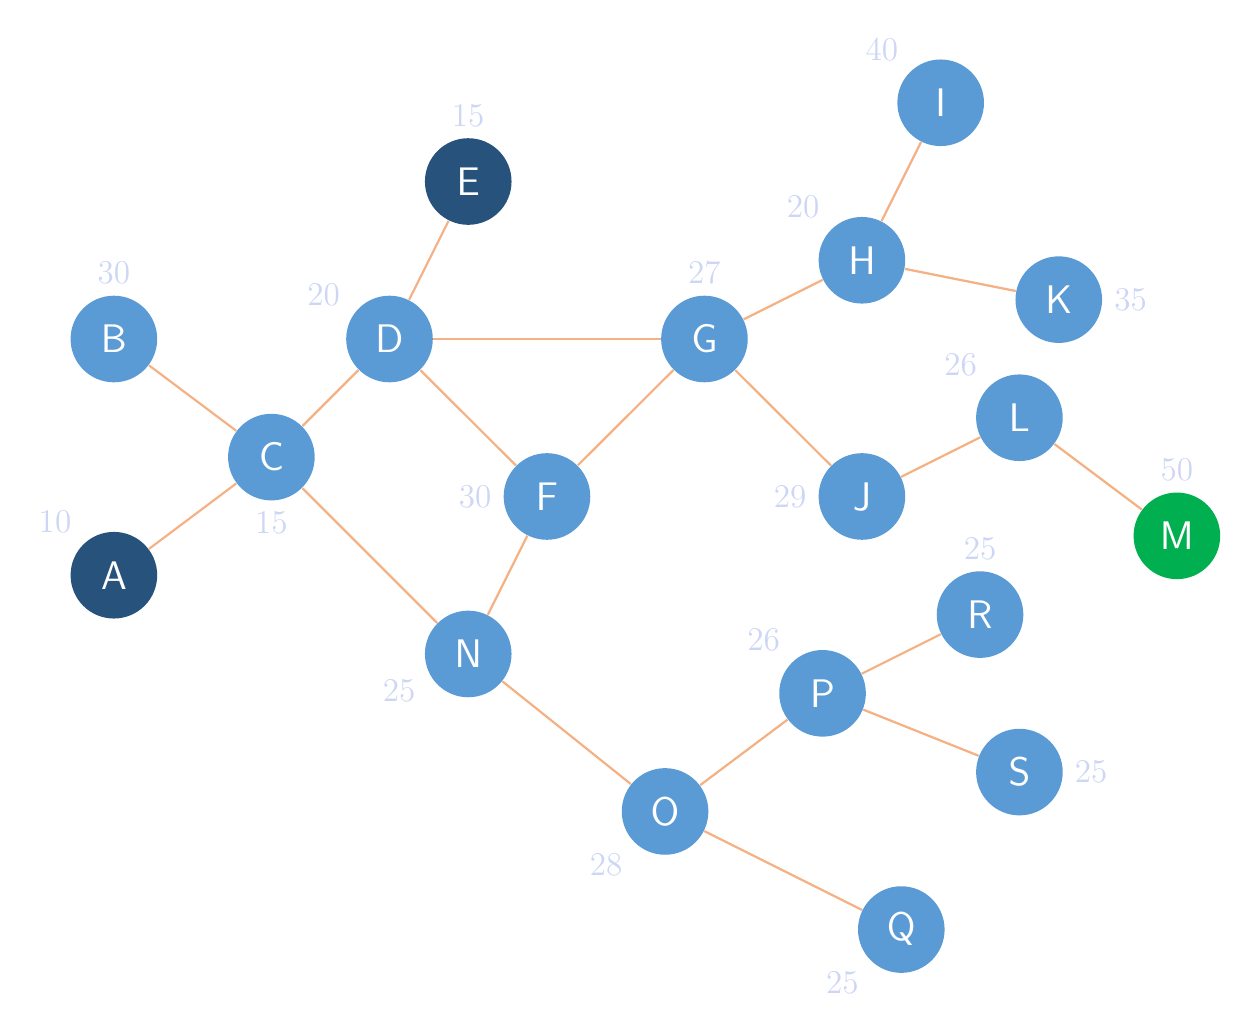
\begin{tikzpicture}[
	scale=1, % Adjust scale for overall spacing
	% Style for the heuristic labels outside the nodes
	every label/.style={
		text=TextPrimary, 
		font=\large, 
		inner sep=4pt
	},
	% Styles for the different node colors
	node light/.style={
		circle, 
		fill=NodeLight, 
		text=white, 
		minimum size=11mm, 
		font=\Large\sffamily
	},
	node dark/.style={
		circle, 
		fill=NodeDark, 
		text=white, 
		minimum size=11mm, 
		font=\Large\sffamily
	},
	node green/.style={
		circle, 
		fill=NodeGreen, 
		text=white, 
		minimum size=11mm, 
		font=\Large\sffamily
	},
	% Style for the unweighted connecting edges
	edge/.style={
		draw=EdgeLine, 
		thick
	}
	]
	
	% ================= NODES =================
	% Syntax: \node[style, label={angle:text}] (ID) at (x, y) {Text inside};
	
	\node[node dark,  label={135:10}] (A) at (-2.0, -1.5) {A};
	\node[node light, label={90:30}]  (B) at (-2.0,  1.5) {B};
	\node[node light, label={270:15}] (C) at ( 0.0,  0.0) {C};
	\node[node light, label={150:20}] (D) at ( 1.5,  1.5) {D};
	\node[node dark,  label={90:15}]  (E) at ( 2.5,  3.5) {E};
	\node[node light, label={180:30}] (F) at ( 3.5, -0.5) {F};
	\node[node light, label={200:25}] (N) at ( 2.5, -2.5) {N};
	\node[node light, label={90:27}]  (G) at ( 5.5,  1.5) {G};
	\node[node light, label={135:20}] (H) at ( 7.5,  2.5) {H};
	\node[node light, label={135:40}] (I) at ( 8.5,  4.5) {I};
	\node[node light, label={0:35}]   (K) at (10.0,  2.0) {K};
	\node[node light, label={180:29}] (J) at ( 7.5, -0.5) {J};
	\node[node light, label={135:26}] (L) at ( 9.5,  0.5) {L};
	\node[node green, label={90:50}]  (M) at (11.5, -1.0) {M};
	\node[node light, label={225:28}] (O) at ( 5.0, -4.5) {O};
	\node[node light, label={135:26}] (P) at ( 7.0, -3.0) {P};
	\node[node light, label={225:25}] (Q) at ( 8.0, -6.0) {Q};
	\node[node light, label={90:25}]  (R) at ( 9.0, -2.0) {R};
	\node[node light, label={0:25}]   (S) at ( 9.5, -4.0) {S};
	
	% ================= EDGES =================
	\draw[edge] (A) -- (C);
	\draw[edge] (B) -- (C);
	\draw[edge] (C) -- (D);
	\draw[edge] (C) -- (N);
	\draw[edge] (D) -- (E);
	\draw[edge] (D) -- (G);
	\draw[edge] (D) -- (F);
	\draw[edge] (F) -- (G);
	\draw[edge] (F) -- (N);
	\draw[edge] (G) -- (H);
	\draw[edge] (G) -- (J);
	\draw[edge] (H) -- (I);
	\draw[edge] (H) -- (K);
	\draw[edge] (J) -- (L);
	\draw[edge] (L) -- (M);
	\draw[edge] (N) -- (O);
	\draw[edge] (O) -- (P);
	\draw[edge] (O) -- (Q);
	\draw[edge] (P) -- (R);
	\draw[edge] (P) -- (S);
	
\end{tikzpicture}


\bigskip
\textcolor{AccentCyan}{\rule{\linewidth}{0.4pt}}

%%%%%%%%%%%%%%%%%%%%%%%%%%%%%%%%%%%%%%%%%%%%%%%%%%%%%%%%%%%%%%%%%%%%%%%%%%%%%%%%%%%%%%%%%%%%%%
\section{\textcolor{AccentGold}{سوال چهارم}}
می‌خواهیم مساله مرتب‌سازی اعداد صحیح متمایز را با الگوریتم‌های جستجوی محلی حل کنیم (یک عدد ثابت در نظر گرفته شده است). هر وضعیت به صورت یک دنباله از اعداد صحیح نمایش داده می‌شود و تنها عمل مجاز در هر وضعیت، جابه‌جایی دو عنصر همسایه در این دنباله عددی می‌باشد. برای مثال دو عمل مجاز در یک وضعیت می‌تواند به صورت \lr{(i,i+1)} و \lr{(i+1,i+2)} باشند.

\begin{enumerate}
	\item[(الف)] در هر وضعیت، چه تعداد وضعیت منحصر به فرد از طریق انجام اعمال مجاز می‌توان به دست آورد؟
	
	\item[(ب)] یک تابع هدف برای این مساله تعریف کنید. فرض کنید که هدف کمینه کردن تابع هدف می‌باشد. تابع شما باید بر اساس مقایسه عناصر در یک وضعیت باشد.
	
	\item[(ج)] آیا تابع هدف شما، مینیمم محلی دارد؟ توضیح دهید.
	
	\item[(د)] فرض کنید که $n=5$ و وضعیت اولیه به صورت \lr{[5,1,4,2,3]} باشد. وضعیت دو مرحله جستجو از این وضعیت را به همراه مقادیر تابع هدف طراحی شده، در هنگام استفاده از هریک از الگوریتم‌های جستجوی زیر بنویسید.
	\begin{itemize}
		\item الگوریتم تپه‌نوردی
		\item الگوریتم سرد کردن تدریجی (\lr{Simulated Annealing}) (مقدار دما را نیز انتخاب کنید)
	\end{itemize}
	
\end{enumerate}

\bigskip
\textcolor{AccentCyan}{\rule{\linewidth}{0.4pt}}
%%%%%%%%%%%%%%%%%%%%%%%%%%%%%%%%%%%%%%%%%%%%%%%%%%%%%%%%%%%%%%%%%%%%%%%%%%%%%%%%%%%%%%%%%%%%%%


\section{\textcolor{AccentGold}{سوال پنجم}}

شکل روبه‌رو نمونه‌ای از مسئله ۸-پازل با حالت آغازین در سمت چپ و حالت نهایی در سمت راست نشان داده شده است. حالت‌ها به صورت زیر هستند:

$$
\quad
\begin{bmatrix}
	3 & 8 & 2 \\
	4 & 6 & 1 \\
	5 & \_ & 7
\end{bmatrix}
\qquad
\quad
\begin{bmatrix}
	1 & 2 & 3 \\
	4 & 5 & 6 \\
	7 & 8 & \_
\end{bmatrix}
$$

\begin{enumerate}
	\item[(الف)] اگر برای حل این مسئله از روش \lr{Hill Climbing} با استفاده از تابع هزینه (\lr{cost}) مجموع فواصل منهتن اعداد تا محل نهایی‌شان استفاده کنیم، آیا لزوماً جواب بهینه به‌دست می‌آید؟ جواب غیر بهینه چگونه است؟ توضیح دهید. (فرض کنید همسایه‌ها همان همسایه‌های یک وضعیت باشند که با اعمال یک کنش (\lr{action}) معتبر به‌دست می‌آیند.)
	
	\item[(ب)] آیا روش بالا معادل با جستجوی اول بهترین حریصانه (\lr{Greedy Best-First Search}) با تابع هیوریستیک معادل با تابع هزینه است؟ توضیح دهید.
\end{enumerate}

\bigskip
\bigskip
\textcolor{AccentCyan}{\rule{\linewidth}{0.4pt}}

% Add more sections as needed...

\end{document}
